En esta sección se detallan las especificaciones de los casos de uso identificados para el proyecto. 

Los casos de uso son descripciones de las interacciones entre los actores y el sistema y son fundamentales para la definición de los requisitos funcionales del mismo.

La especificación de cada caso de uso se ha basado en las recomendaciones de Cockburn \cite{cockburn2000writing}. Cada caso de uso incluye los siguientes elementos:
\begin{itemize}
    \item \textbf{Nombre del caso de uso}: un nombre corto y descriptivo.
    \item \textbf{Descripción}: una descripción general del caso de uso.
    \item \textbf{Actores principales}: los actores que inician el caso de uso.
    \item \textbf{Actores secundarios}: los actores que participan en el caso de uso, pero no lo inician.
    \item \textbf{Precondiciones}: las condiciones que deben cumplirse antes de que el caso de uso pueda comenzar.
    \item \textbf{Postcondiciones}: las condiciones que deben cumplirse al finalizar el caso de uso.
    \item \textbf{Disparadores}: los eventos que inician el caso de uso.
    \item \textbf{Escenario principal}: la secuencia de pasos que describe la interacción entre los actores y el sistema.
    \item \textbf{Escenarios alternativos}: descripciones de las ramificaciones del escenario principal.
    \item \textbf{Situaciones de error}: descripciones de las situaciones en las que el caso de uso puede fallar.
\end{itemize}
% https://www-public.imtbs-tsp.eu/~gibson/Teaching/Teaching-ReadingMaterial/Cockburn00.pdf


Los casos de uso están organizados en secciones según el actor que los inicie. Los actores han sido previamente identificados y descritos en el apartado denominado
\coloredUnderline{\hyperlink{sec:6_1-Identificacion_actores}{\ref*{sec:6_1-Identificacion_actores} \nameref*{sec:6_1-Identificacion_actores}}}.

En la figura \coloredUnderline{\hyperlink{fig:diagrama_contexto}{Figura \ref*{fig:diagrama_contexto}: \nameref*{fig:diagrama_contexto}}}
se muestra el diagrama de contexto del sistema, que representa las interacciones entre los actores y el sistema. 
Este diagrama introduce los casos de uso que se describen en las siguientes secciones.

\begin{figure}[H]
    \centering
    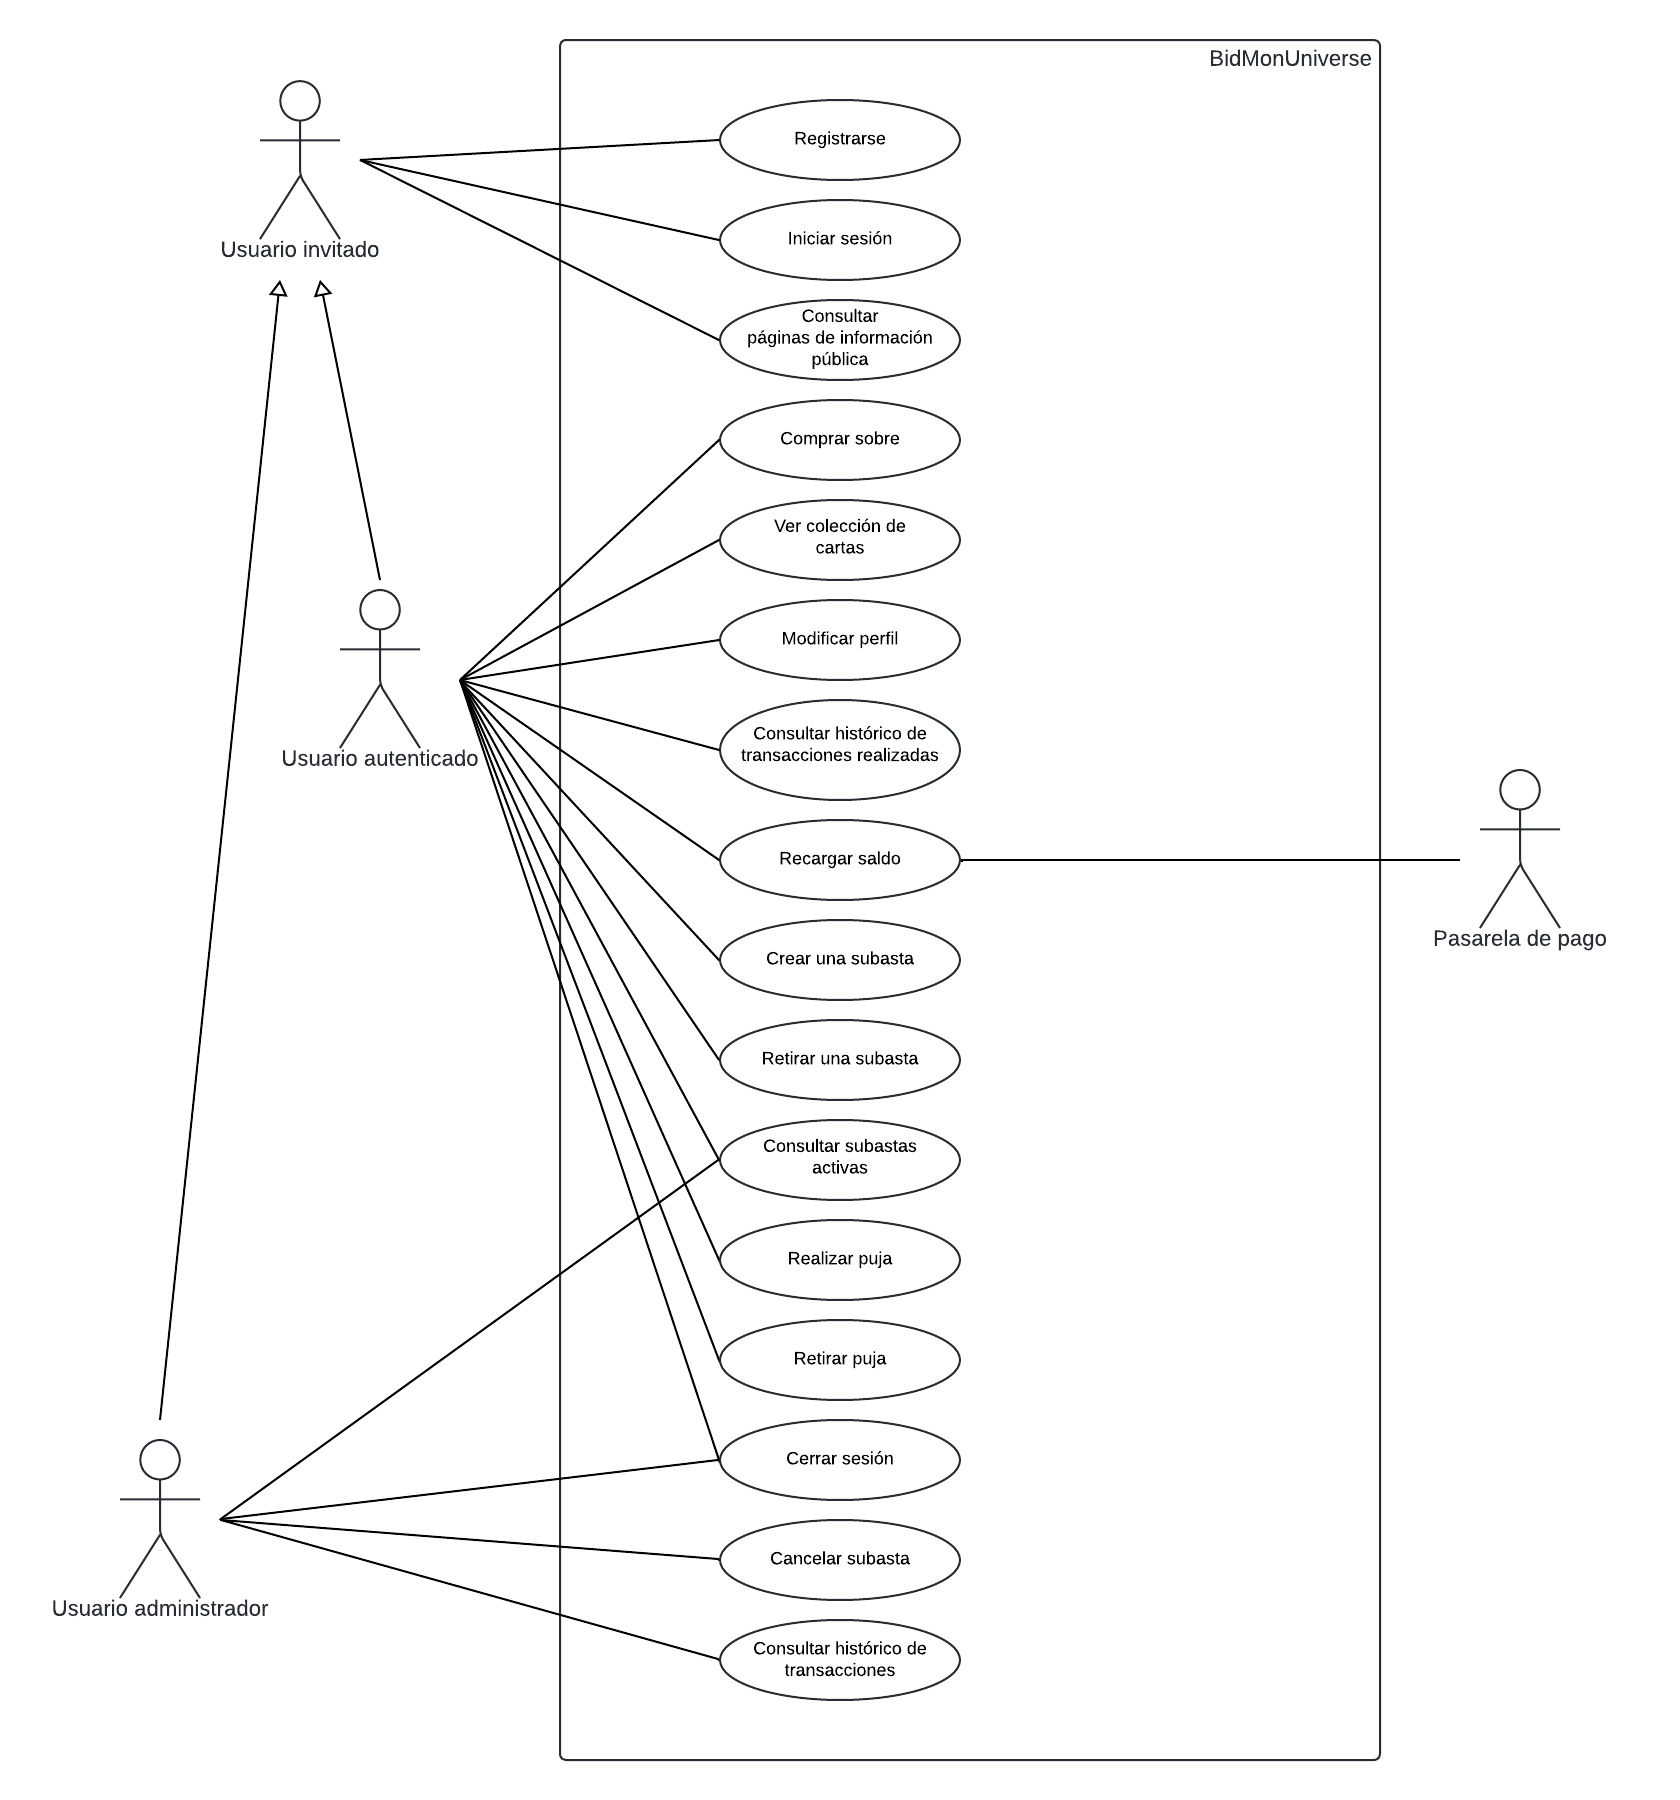
\includegraphics[width=0.9\textwidth]{figures/6-Analisis/6-Casos-uso/6_Diagrama-contexto.png}
    \caption{Diagrama de contexto del sistema}
    \label{fig:diagrama_contexto}
\end{figure}

\subsection{Casos de uso. Usuario invitado}

\begin{figure}[H]
  \centering
  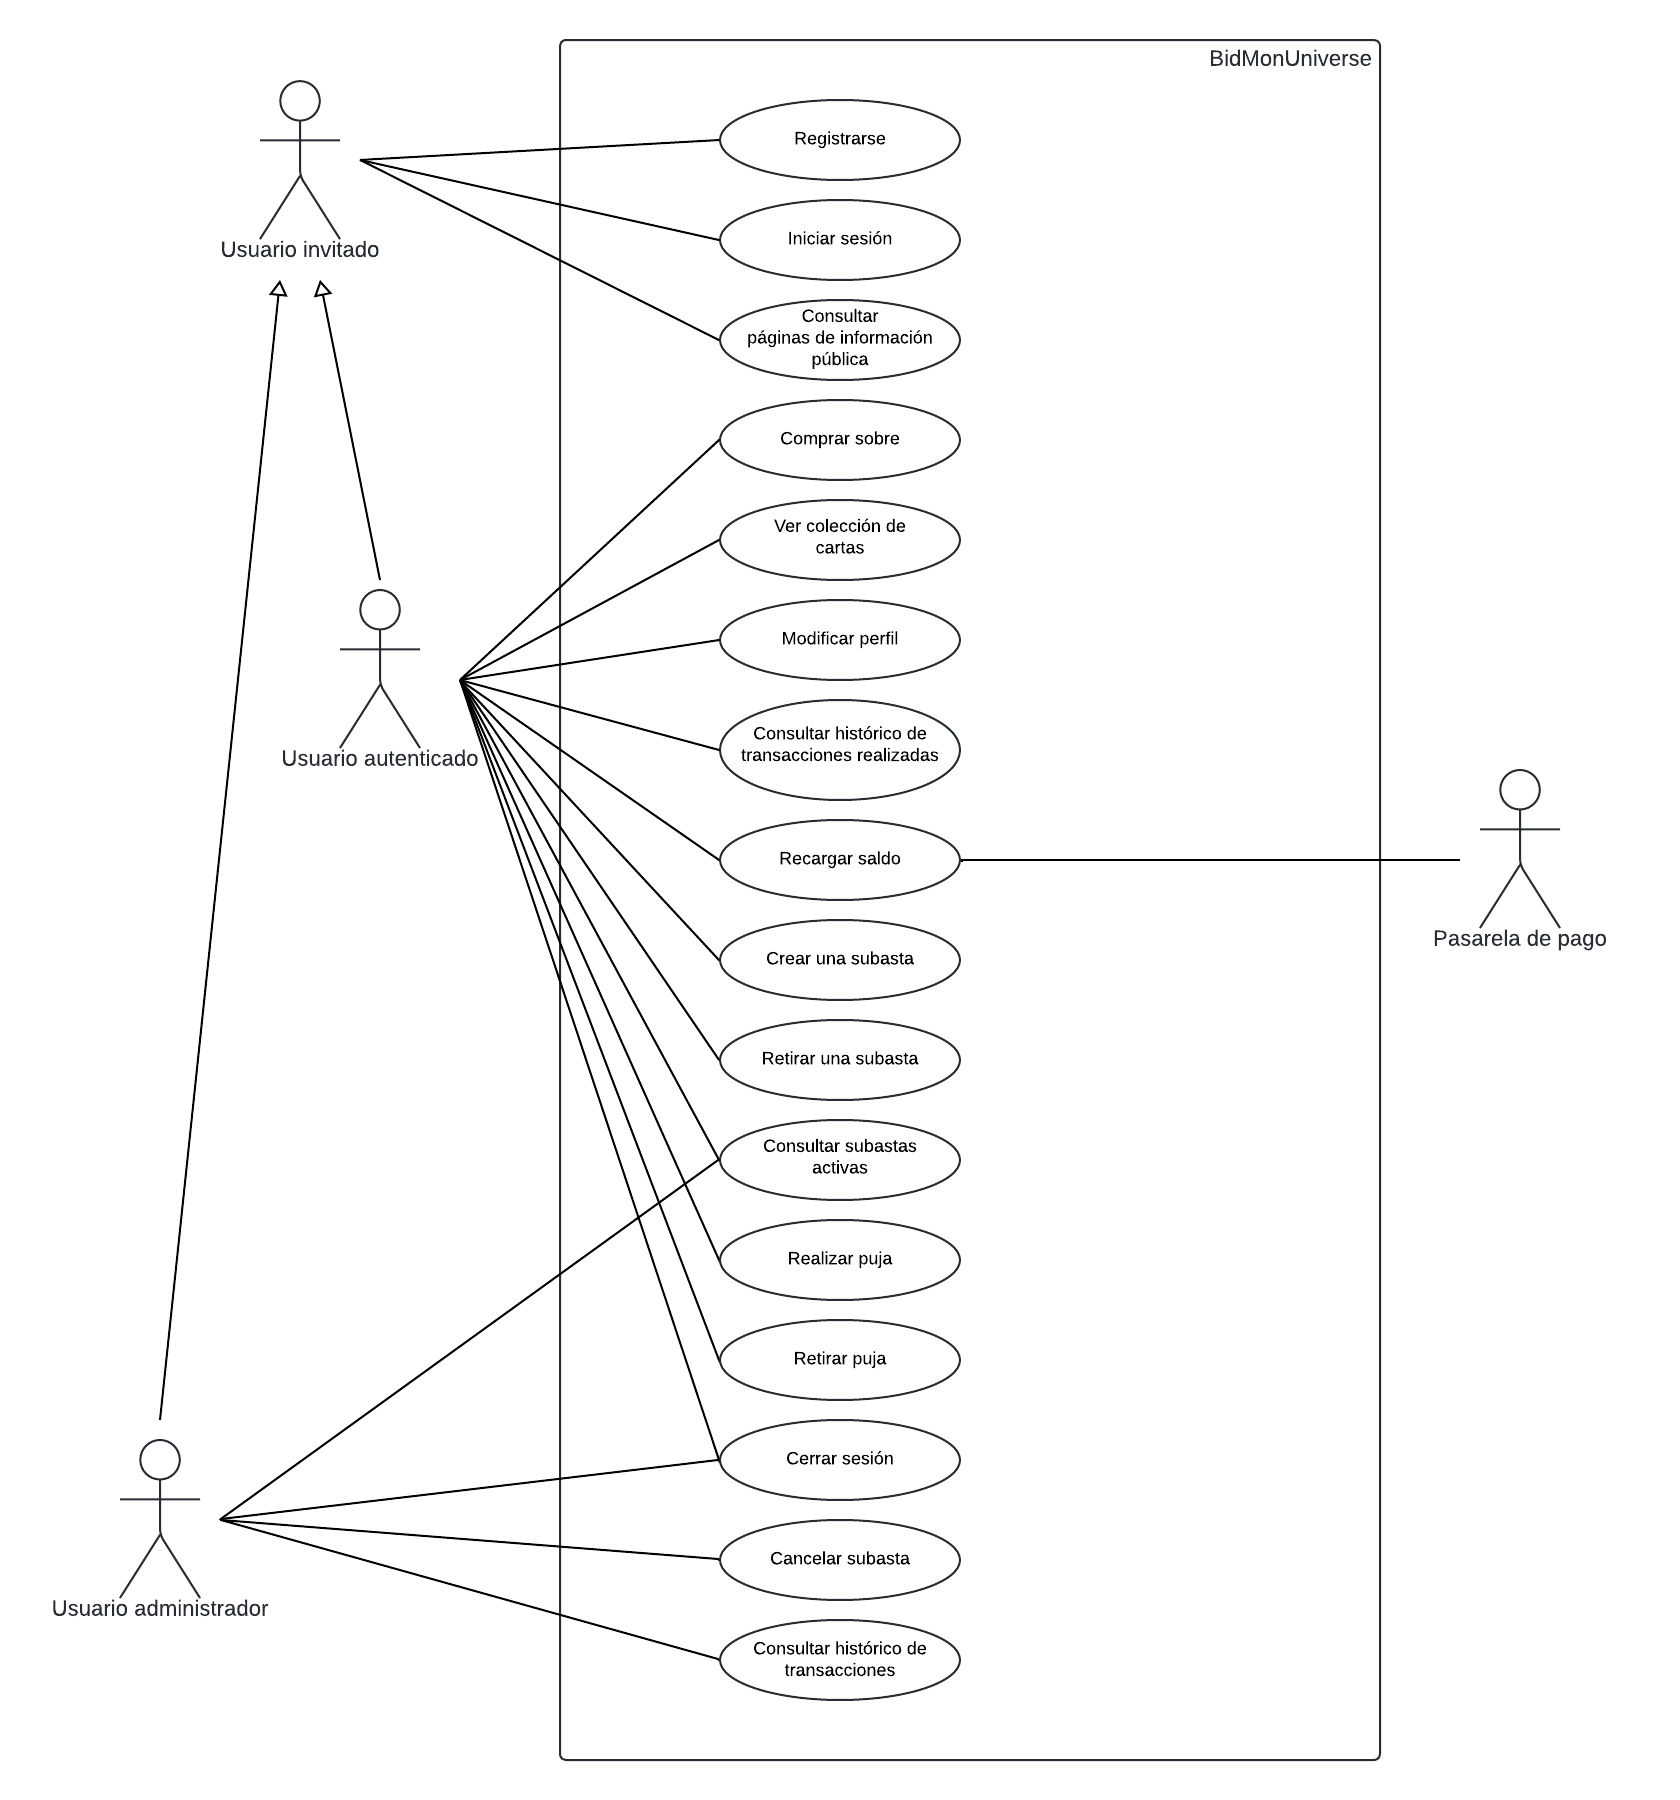
\includegraphics[width=0.9\textwidth]{figures/6-Analisis/6-Casos-uso/6_Diagrama-contexto.png}
  \caption{Diagrama de contexto del sistema}
  \label{fig:diagrama_contexto}
\end{figure}

\subsection{Casos de uso. Usuario invitado}
\begin{longtable}{
>{\columncolor{lightgreen!20}}p{4cm}
p{12cm}
}
\caption{Caso de Uso: Registro} \label{table:usecase} \\
\toprule
\rowcolor{darkgreen!50}
\textbf{Caso de uso} & \multicolumn{1}{>{\columncolor{darkgreen!50}\centering\arraybackslash}p{12cm}}{\textbf{REGISTRO}} \\
\endfirsthead

\multicolumn{2}{c}%
{{ \tablename\ \thetable{} -- continuación de la página anterior}} \\
\toprule
\rowcolor{darkgreen!50}
\textbf{Caso de uso} & \multicolumn{1}{>{\columncolor{darkgreen!50}\centering\arraybackslash}p{12cm}}{\textbf{REGISTRO}} \\
\midrule
\endhead

\midrule
\multicolumn{2}{r}{{Continúa en la siguiente página...}} \\ 
\endfoot

\bottomrule
\endlastfoot

\midrule
Descripción & Un usuario invitado se puede registrar en el sistema para poder acceder a las funcionalidades del mismo. \\
\midrule
Actores principales & Usuario invitado \\
\midrule
Actores secundarios &  \\
\midrule
Precondiciones & El usuario no debe estar registrado en el sistema. \\
\midrule
Postcondiciones & \begin{itemize}[nosep,leftmargin=*]
  \item Se crea un nuevo registro en la base de datos con los datos del usuario.
  \item Se notifica al usuario que su registro ha sido exitoso.
  \item Se redirige al usuario a la página de inicio de sesión.
\end{itemize} \\
\midrule
Disparadores & El usuario hace clic en el botón de registro. \\
\midrule
Escenario principal & \begin{enumerate}[nosep,leftmargin=*]
  \item El sistema muestra el formulario de registro.
  \item El usuario completa el formulario con sus datos personales.
  \item El usuario hace clic en el botón de registro.
  \item El sistema valida los datos del formulario.
  \item El sistema crea un nuevo registro en la base de datos con los datos del usuario.
  \item El sistema notifica al usuario que su registro ha sido exitoso.
  \item El sistema redirige al usuario a la página de inicio de sesión.
\end{enumerate} \\
\midrule
Escenarios alternativos & 
\begin{itemize}[nosep,leftmargin=*]
  \item Escenario alternativo 1. El usuario cancela el registro.
  \begin{enumerate}[nosep,leftmargin=*]
      \item El usuario hace clic en otro enlace.
      \item El sistema no crea el registro y redirige al usuario a la página correspondiente.
  \end{enumerate}
  \item Escenario alternativo 2. El usuario ya está registrado en el sistema.
  \begin{enumerate}[nosep,leftmargin=*]
      \item El sistema muestra un mensaje de error.
      \item El sistema no crea el registro y redirige al usuario de nuevo al formulario de registro.
  \end{enumerate}
  \item Escenario alternativo 3. El usuario no completa el formulario correctamente.
  \begin{enumerate}[nosep,leftmargin=*]
      \item El sistema muestra un mensaje de error con los campos que no se han completado correctamente.
      \item El sistema no crea el registro y redirige al usuario de nuevo al formulario de registro.
  \end{enumerate}
\end{itemize} \\
\midrule
Situaciones de error & \begin{itemize}[nosep,leftmargin=*]
  \item Error 1. Error de conexión a la base de datos.
  \begin{enumerate}[nosep,leftmargin=*]
      \item El sistema muestra un mensaje de error.
      \item El sistema redirige al usuario de nuevo al formulario de registro.
  \end{enumerate}
\end{itemize} \\
\end{longtable}